\documentclass[12pt]{amsart}
\usepackage{amsmath, amssymb, amsthm}
\usepackage[margin=2.5cm]{geometry}
\usepackage{hyperref}
\usepackage{xurl}
\usepackage{booktabs}
\usepackage{graphicx}

\newtheorem{observation}{Observation}
\newtheorem{derivation}[observation]{Derivation}
\newtheorem{remark}[observation]{Remark}

\title[Arithmetic satellites of the Riemann zero comb]{Arithmetic
satellites of the Bragg comb of the Riemann zero lattice:\\ residue
classes, characters, and a blind test of the Bogomolny--Keating mirror
law}

\author{U\u{g}ur Sezen}
\address{Independent researcher, Istanbul, Turkey}
\email{usezen@aof.anadolu.edu.tr}

\date{\today}

\begin{document}

\begin{abstract}
Companion notes found that the per-gap response of the Riemann zeros to
the prime waves of the explicit formula is partly cancelled by the waves
beyond any finite truncation, through a kernel concentrated on the Bragg
comb of the lattice of gap midpoints. We study the satellites of that
comb. Their positions form a height-independent grid
$\Delta\omega = \omega - \log(t/2\pi) = \log(a/b)$. A stationary-phase
analysis predicts that a satellite reads the residue class of the
contributing prime power modulo $a$: the naive prediction of rotating
class phases fails, while the refined law --- class shares
$\cos(2\pi rb/a)/\mu(a)$ --- passes a blind test at $+\log 10$ (two other
satellites follow its signs but exceed its magnitudes). On the zeros of
real Dirichlet $L$-functions, satellites involving a prime that divides
the conductor vanish, and the cancellation keeps the sign of the zeta
case for both parities. The Euler product of the Bogomolny--Keating pair
correlation gives the satellite amplitudes in closed form. It implies a
mirror law --- on the negative side the envelope is exactly $1/x$ at
$\Delta\omega = -\log x$ --- which a pre-registered blind test in a
previously unexamined band confirms at $1.023 \pm 0.023$ of the
prediction, excluding a line-density rival by more than $12\sigma$.
Coefficients with a positive exponent are transferred with a factor
below one that relaxes towards one with height (exponent
$1.36 \pm 0.21$ over three windows; a constant is excluded at
$6.4\sigma$); since the ratios-conjecture pair correlation has no such
term, this is a property of our mixed zero--prime observable. Nothing
here bears on a proof of the Riemann Hypothesis.
\end{abstract}

\maketitle

\section{Introduction}

The explicit formula writes the fluctuating part of the zero counting
function as a sum of prime waves,
\begin{equation}\label{eq:S}
N(t) = \bar N(t) + S(t), \qquad
S(t) = -\sum_{q} a_q \sin(\omega_q t), \qquad
a_q = \frac{\Lambda(q)}{\pi\sqrt{q}\,\log q},\quad \omega_q = \log q,
\end{equation}
the sum running over prime powers $q$. Companion notes
\cite{companion1,companion2,companion3,companion4} measured how the local
statistics of the zeros respond to these waves: an amplitude channel and a
zero-displacement channel, each a one-variable law in
$\tau = \log q/L$, $L = \log(t/2\pi)$ \cite{companion2,companion3}, and
--- in \cite{companion4} --- the diffraction pattern of the lattice of gap
midpoints, with arithmetic spots at $\log p^k$ and Bragg combs at
multiples of the mean density frequency $\omega = L$.

This note is about the neighbourhood of the first comb. Any measurement
of the response to the waves must truncate the sum \eqref{eq:S} at some
$\tau_c$; the waves beyond the truncation do not simply add noise but
\emph{cancel} a fixed fraction of the interference ("mixing") among the
waves inside it, at a phase of exactly $180^\circ$. Resolving that
cancellation by the frequency $\omega'$ of the cancelling waves gives a
kernel $\kappa(\omega')$, and the kernel turns out to be concentrated on
the comb $\omega' = L$ and on a family of \emph{satellites}
$\omega' = L + \log(a/b)$. The satellites carry arithmetic: which of them
light up, with which amplitude and with which internal structure is
decided by the M\"obius function, by residue classes, by Dirichlet
characters and, as we show, by the Euler product of the
Bogomolny--Keating pair correlation \cite{BK95,BK96,Bog07,CS07}.

Satellites at $\log(a/b)$ are the fingerprint, in the zero lattice, of
the arithmetic terms of the pair correlation that are conjectural in the
regime $\alpha > 1$ of Montgomery's form factor \cite{Mont73,Rod13}; the
single-point analogue is the Landau--Gonek formula for
$\sum_\gamma x^{i\gamma}$ \cite{Landau12,Gonek93,Fujii89,DHPC26}, and
the structure factor of the primes themselves has Bragg peaks with
heights $\mu(q)^2/\varphi(q)^2$ at rational frequencies
\cite{ZMT18,TZdCI18}. We do not claim that the mechanism is new; what the
note adds is a measurement programme on the zero side, organised as a
sequence of pre-registered tests in which each prediction, its
thresholds and its death conditions were frozen and published before the
data were looked at, and in which failed predictions are reported next to
the successful ones. We call a test \emph{pre-registered} when the
predictions, thresholds and analysis definitions were fixed and published
(with a time stamp) before the relevant quantity was computed, and
\emph{blind} when, in addition, the data region it uses had never been
displayed or searched. Results found after looking at the data are marked
\emph{post hoc}.

Section~\ref{sec:obs} defines the observable. Section~\ref{sec:pos}
shows that the satellite positions are height-independent.
Section~\ref{sec:classes} derives the selection rules from stationary
phase and tests the residue-class law. Section~\ref{sec:L} carries the
analysis to Dirichlet $L$-functions. Section~\ref{sec:BK} derives the
amplitudes from the Bogomolny--Keating Euler product and reports the
blind test of the mirror law. Section~\ref{sec:height} measures the
height dependence of the positive-exponent coefficients, and
Section~\ref{sec:open} lists open problems.

\section{The observable}\label{sec:obs}

\subsection*{Data} We use A.~M.~Odlyzko's table of the first
$2\times10^6$ zeros \cite{OdlyzkoTables,Odl87} and three windows of consecutive zeros:
\emph{alt}, the zeros $2\times10^4$--$2\times10^5$ ($1.8\times10^5$ gaps,
mean $L = 9.34$; used only in Section~\ref{sec:height}); \emph{low}, the zeros $2\times10^5$--$5\times10^5$
($3\times10^5$ gaps, $L = 10.48$, $t \in [1.40, 3.19]\times10^5$); and
\emph{last}, the top $3\times10^5$ gaps of the table ($L = 12.03$).

\subsection*{The per-gap identity}
Let $t_n$ be the ordinates, $g_n = t_{n+1} - t_n$ the gaps and
$m_n = (t_n + t_{n+1})/2$ the midpoints. Differencing \eqref{eq:S} over
one gap, $N(t_{n+1}) - N(t_n) = 1$, gives for the unfolded gap deviation
\begin{equation}\label{eq:ds}
\delta_n := \frac{g_n L(m_n)}{2\pi} - 1
= \sum_q 2a_q \sin\!\Big(\frac{\omega_q g_n}{2}\Big)\cos(\omega_q m_n),
\end{equation}
up to the curvature of $\bar N$ over one gap. Every wave enters the gap
through its difference across the gap, sampled at the midpoint.

\subsection*{Truncation, mixing and cancellation}
Truncate \eqref{eq:ds} to the \emph{window} $\tau_q \le \tau_c = 0.86$
and project the truncated series onto each window line,
$c_q = 2\langle \delta^{(\tau_c)}_n e^{-i\omega_q m_n}\rangle_n$. The
projection splits into the line's own contribution and a \emph{mixing}
term, $c_q = c_q^{\mathrm{self}} + \mathrm{mix}_q$, produced by the other
window lines. On a uniform grid distinct frequencies would be orthogonal;
here the waves are sampled at the midpoints $m_n$ and through the gaps
$g_n$, which are themselves displaced by the primes, so the Gram couplings
between wave columns are values of the midpoint structure factor
$\hat G(\omega_q - \omega_{q'})$ \cite{companion4} and do not vanish. The
lines beyond the window add a further projection $\Delta_q$. Regressing
it on the mixing over a pool of lines,
\begin{equation}\label{eq:zeta}
\zeta = \frac{\sum_{q\in\mathcal P} \Delta_q\,\overline{\mathrm{mix}_q}}
{\sum_{q\in\mathcal P}|\mathrm{mix}_q|^2},
\qquad \mathcal P = \{q: \tau_q \in [0.45, 0.86)\},
\end{equation}
gives $\zeta = 0.333\angle180^\circ$ in the low window and
$0.329\angle180^\circ$ in the last: the waves beyond the window cancel a
third of the in-window mixing, at exactly opposite phase, independently
of height.

\subsection*{The kernel}
Resolve $\Delta_q$ by the frequency $\omega'$ of the lines that produce
it. The window is cut into blocks $b$ of consecutive gaps with mean
$L_b$; each line $q'$ is assigned, in each block, to the slice
$j = \lfloor(\omega_{q'} - L_b)/0.025 + \tfrac12\rfloor$ of the
\emph{block-local} axis $\Delta\omega = \omega' - L_b$; the slice's
per-gap series $\delta^{(b,j)}_n = \sum_{q'\in j} 2a_{q'}\sin(\omega_{q'}g_n/2)\cos(\omega_{q'}m_n)$
is projected onto the pool lines within the block,
$C_{b,j}(q) = 2\langle \delta^{(b,j)}_n e^{-i\omega_q m_n}\rangle_{n\in b}$, and
\begin{equation}\label{eq:K}
K_{b,j} = \frac{\sum_{q\in\mathcal P} C_{b,j}(q)\,\overline{\mathrm{mix}_q}}
{\sum_{q\in\mathcal P}|\mathrm{mix}_q|^2}, \qquad
\kappa_j = -\,\frac{\sum_{b} n_b\,\mathrm{Re}\,K_{b,j}}{\sum_b n_b},
\end{equation}
the sums over $b$ running over the blocks that cover slice $j$ entirely
so that $\kappa > 0$ is cancellation-directed and
$\sum_j K_j$ reproduces the beyond-window part of $\zeta$ (to machine
precision). For slices inside the window the slice's own contribution is
removed from the truncated series before the mixing is formed, which
makes the definition identical to the beyond-window one. Uncertainties
are jackknife errors over eight contiguous groups of blocks; $z$ denotes a
signed ratio to that error and ``$n\sigma$'' its magnitude. Where a
decision rule uses $\sigma_{\mathrm{eff}}$, the jackknife error has been
inflated by a factor ($1.2$--$1.6$) calibrated, before the data were seen,
on synthetic replicas processed by the same pipeline.

\subsection*{Line shape}
A satellite at $\Delta\omega = \log r$ is produced, gap by gap, at
$\omega' = L(m_n) + \log r$; within a block it is therefore smeared over
the spread of $L(m_n)$. With eight blocks per window this spread is
$0.07$--$0.15$, which is larger than the spacing of many satellites; with
32 blocks, or blocks of equal width $\Delta L \le 0.03$ (used from
Section~\ref{sec:BK} on), it is $0.017$--$0.041$. The line shape
$h(j; r)$ follows parameter-free from the distribution of $L(m_n)$ in each
block, and all amplitude measurements of Sections~\ref{sec:BK}
and~\ref{sec:height} are linear fits of the profile $\kappa_j$ with these
shapes and a linear baseline.

\section{Positions: a height-independent grid}\label{sec:pos}

Mapped against the frequency of the cancelling lines and the pool band,
the kernel has a simple structure. It is $77\%$ rank-one (a pre-registered threshold of $80\%$ for a
rank-one mechanism was not met), with a band factor at
$180^\circ\pm5^\circ$ in every pool band, and its structure sits on a comb in $\tau'$: the Bragg
line $\tau' = 1$ and satellites; the strongest feature beyond the Bragg
line, at $\tau' \in (1.05, 1.10]$, is $96\%$ carried by the satellites of
$2$ and $3$.

The natural axis is not $\tau'$ but $\Delta\omega$.

\begin{observation}[Height independence; pre-registered]
In the low window ($L = 10.48$), with the definitions frozen on the last
window ($L = 12.03$), the block-median kernel peaks fall at
$\Delta\omega = 0.025$, $0.725$, $1.113$ and $1.800$, against the targets
$0$, $\log2 = 0.693$, $\log3 = 1.099$ and $\log 6 = 1.792$, all within
$\pm0.05$, and far from the positions $0.604$, $0.957$, $1.562$ predicted
by a fixed-$\tau'$ comb; the block-to-block slopes are zero, where a
fixed-$\tau'$ reading requires $-1$.
\end{observation}

Post hoc, the two windows' profiles overlap on the $\Delta\omega$ axis
with correlation $0.980$, against $0.002$ on the $\tau'$-scaled axis.

Figure~\ref{fig:pos} shows the overlap. The cancelling waves are those
whose frequency exceeds the local density frequency by the logarithm of a
rational number.

\begin{figure}[t]
\centering
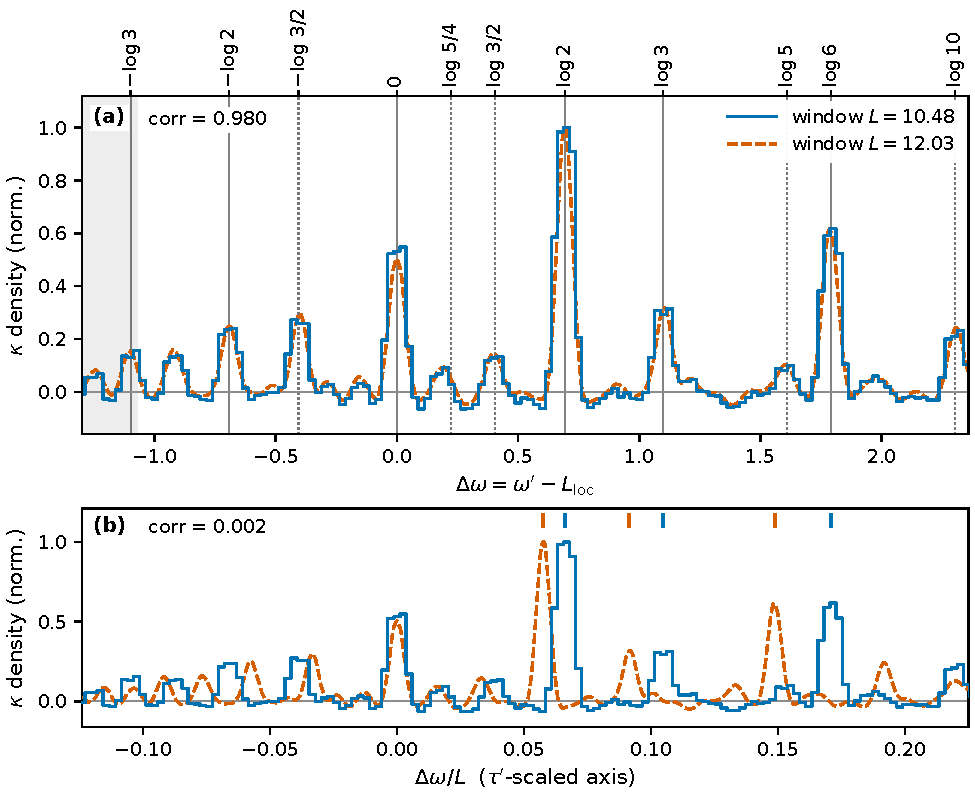
\includegraphics[width=0.95\textwidth]{fig_n7_positions_en.pdf}
\caption{\label{fig:pos}\textbf{Satellite positions are universal in $\Delta\omega$.}
  (a)~Pooled cancellation-kernel density $\kappa$, normalized to its maximum on
  $-1.3\le\Delta\omega\le2.3$, versus $\Delta\omega=\omega'-L_{\rm loc}$ for two windows of
  zeros, $L=10.48$ (solid, bins of $0.025$) and $L=12.03$ (dashed, $\tau'$ bins of width
  $0.060$ in $\omega$); vertical lines mark satellites at $\log(a/b)$, solid for the
  pre-registered targets $0,\pm\log2,\pm\log3,\log6$ and dotted for the other satellites
  that are bright in both windows.
  In the $L=10.48$ window the pre-registered block-median peaks lie at $0.025$, $0.725$,
  $1.113$ and $1.800$ (targets $0,\log2,\log3,\log6$), each within $0.05$ of its target and
  away from the $\tau'$-fixed alternatives $0.604$, $0.957$, $1.562$, and the two profiles
  correlate at $0.980$.
  (b)~On the $\tau'$-scaled axis $\Delta\omega/L$ the same profiles no longer coincide
  (correlation $0.002$; ticks mark $\log n/L$ for $n=2,3,6$ in each window).
  The shaded strip $\Delta\omega<-1.07$ is only partly covered by the eight blocks of the
  $L=10.48$ window.}
\end{figure}

\section{Selection rules and residue classes}\label{sec:classes}

\begin{derivation}[Stationary phase]\label{der:sp}
The midpoints satisfy $N(m_n) = n$ exactly, with
$2\pi\bar N(t) = tL(t) - t + 7\pi/4$. Hence
$e^{i\omega' m_n} = e^{i(\omega' m_n - 2\pi\bar N(m_n))}\,e^{-2\pi i S(m_n)}$,
and by the Jacobi--Anger expansion
$e^{-2\pi i S} = \prod_q \sum_{k} J_k(2\pi a_q)\,e^{ik\omega_q t}$. The term
labelled $\{k_q\}$ has phase
$\phi(t) = (\omega' + \sum_q k_q\omega_q)t - 2\pi\bar N(t)$ with a
stationary point at $L(t^*) = \omega' - \log n$,
$n := \prod_q q^{-k_q}$, which may be rational. Satellites therefore sit at
$\Delta\omega = \log n$, for every height. Writing $n = a/b$ in lowest
terms, $t^* = 2\pi q'b/a$ for a line $q'$ with $\omega' = \log q'$, and the
stationary value of the phase is $2\pi q'b/a$ up to the constant
$-7\pi/4 - \pi/4 \equiv 0$ (the last $-\pi/4$ is the stationary-phase
factor of a phase with $\phi'' = -1/t < 0$). The contribution of a line
depends on $q' \bmod a$.
\end{derivation}

Two predictions follow. (a) \emph{Selection}: prime powers are
equidistributed over the reduced residue classes modulo $a$, so the
coherent sum over lines is a Ramanujan sum, $c_a(1)/\varphi(a) =
\mu(a)/\varphi(a)$ \cite{Apo76}; satellites with $\mu(a) = 0$ vanish.
(b) \emph{Class structure}: empirically the kernel follows the real part
of the midpoint structure factor at $\omega'$ (a proxy that explains
$90$--$95\%$ of it), so it reads the real part of the class phase, and the
share of residue class $r$ in the satellite is
\begin{equation}\label{eq:shares}
s_r = \frac{\cos(2\pi r b/a)}{\mu(a)} .
\end{equation}

The first version of this analysis (without the final $-\pi/4$, and with
the class \emph{phases} rather than their real parts as observable)
predicted that the classes of $+\log 3$ would appear $120^\circ$ apart.
That prediction was pre-registered and \emph{failed}: the two classes of
$+\log 3$ are $-8.6^\circ \pm 3.9^\circ$ apart and carry $0.46$ and $0.54$
of the satellite, statistically indistinguishable from the control
$-\log 3$ ($-0.9^\circ\pm5.5^\circ$). The selection
rule survived: none of nine positions with $\mu(a) = 0$ lights up (the
largest is $+1.6\sigma$), while all six main satellites do
($7.6$--$12.4\sigma$); only three of the nine are, however, consistent
with zero --- the others carry significant \emph{negative} values. The refined law \eqref{eq:shares} was then
pre-registered as a blind test on a satellite never analysed by class.

\begin{observation}[Residue classes of $+\log10$; blind]
The four classes $r = 1, 9, 3, 7 \pmod{10}$ of the satellite
$+\log 10$ (last window) carry the shares
$+0.899\pm0.023$, $+0.902\pm0.017$, $-0.416\pm0.035$, $-0.386\pm0.035$,
against $\cos(2\pi r/10) = +0.809, +0.809, -0.309, -0.309$: all four
signs, at $|z| = 11$--$52$, each within $0.11$ of the prediction. The
controls behave as required: $+\log 3$ splits $0.462/0.538$ and $-\log 3$
(with $a = 1$, no class structure) $0.499/0.501$.
\end{observation}

The class structure of $+\log 7$ has the predicted signs in all four
classes ($|z| = 4.9$--$6.2$) but magnitudes $1.8$--$2.4$ times the
prediction; $+\log 5$, reported without verdict, shows a smaller
stretch ($1.25$--$1.75$). We do not know its origin. A pre-registered attempt to
explain it by a negative kernel floor between satellites failed: away
from satellites the kernel is consistent with zero
($+0.00024\pm0.00017$). The positions with $\mu(a) = 0$ are not exactly
zero either: they carry small negative residues, $9.4\sigma$ below the
empty-window floor in the last window, and of the same size in all three
windows of Section~\ref{sec:height}.

\begin{figure}[t]
\centering
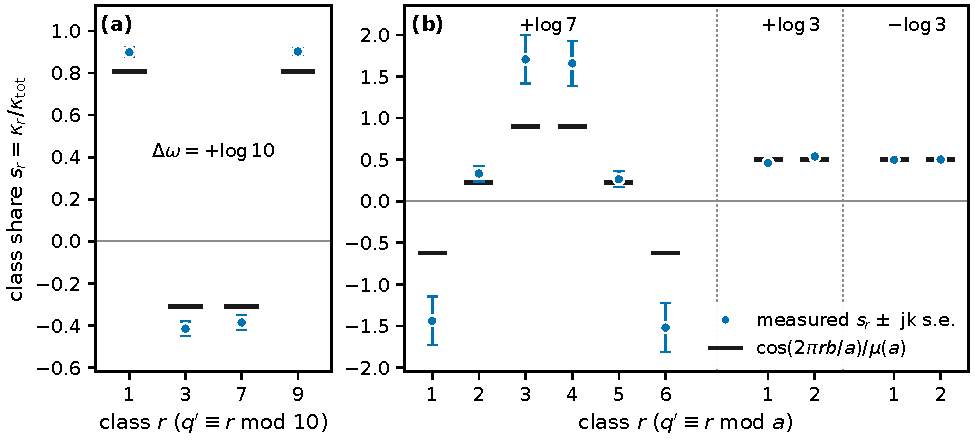
\includegraphics[width=0.95\textwidth]{fig_n7_classes_en.pdf}
\caption{\label{fig:classes}\textbf{Residue-class law of the satellites.}
  Class shares $s_r=\kappa_r/\kappa_{\rm tot}$ of the lines $q'\equiv r\pmod a$ (points,
  8-block jackknife errors) against the blind prediction
  $s_r=\cos(2\pi rb/a)/\mu(a)$ (bars), window $L=12.03$.
  (a)~At $\Delta\omega=+\log10$ all four classes have the predicted sign and lie within
  $0.11$ of the prediction: $s_1=0.899\pm0.023$ and $s_9=0.902\pm0.017$ (predicted $0.809$),
  $s_3=-0.416\pm0.035$ and $s_7=-0.386\pm0.035$ (predicted $-0.309$).
  (b)~At $+\log7$ the signs are again correct ($|z|=4.9$--$6.2$ for $r=1,3,4,6$) but the
  magnitudes are $1.8$--$2.4$ times the prediction, while the controls $+\log3$
  ($0.462/0.538$) and $-\log3$ ($0.499/0.501$, no class structure expected) sit at
  $\tfrac12/\tfrac12$.}
\end{figure}

\section{Dirichlet $L$-functions}\label{sec:L}

For a primitive real character $\chi$ modulo $k$ the counting function has
$L_\chi(t) = \log(kt/2\pi)$ and waves weighted by $\chi(q)$. The
Jacobi--Anger factor of a wave with $\chi(q) = 0$ is trivial, so
satellites $\log(a/b)$ with a prime of $ab$ dividing $k$ are absent. The
stationary point moves to $t^* = 2\pi q'b/(ka)$, the class sum becomes
$\chi(a)\bar\chi(b)\tau(\chi)\mu(a)$ with the Gauss sum $\tau(\chi)$ (not to be confused with
$\tau = \log q/L$), the
character signs cancel against the amplitudes $\chi(a)\chi(b)$, and the
phase of $\tau(\chi)$ (real for even, imaginary for odd $\chi$) combines
with the parity-dependent constant of $\bar N_\chi$ to give a
\emph{real} kernel with the sign of the zeta case for both parities. Two
rival pictures --- one that forgets the conductor in $t^*$ (no
cancellation on the islands) and one that forgets the parity (no
cancellation for odd $\chi$) --- were pre-registered alongside.

\begin{observation}[Characters; pre-registered]
On the zeros of $L(s,\chi)$ for $\chi_4$, $\chi_3$, $\chi_5$ (even),
$\chi_8$ (even) and $\chi_8$ (odd) up to $t \approx 5\times10^4$: all
$21$ satellites forbidden by the conductor are dark in the structure
factor (22 of the 24 allowed ones at $+9.8$ to $+12.1\sigma$, the two
exceptions being $+\log 4$, where $\mu(4) = 0$) and suppressed in the
kernel to a small residue; the
allowed satellites cancel on all five islands, for both parities, with
the zeta sign and a real phase ($180^\circ\pm1.3^\circ$; $z = -55$ to $-82$
for the primary satellite pairs); the even and odd characters modulo $8$ agree to $1.009\pm0.024$.
Both rivals die.
\end{observation}

Two parts of the prediction failed. The forbidden satellites leave a
residue of $3$--$5\%$ of the allowed ones, with opposite sign --- the same
level as the $\mu(a) = 0$ residues of the zeta case. And the predicted
amplitude ratio to zeta at matched $L$, $\sqrt{k}/\varphi(k)$, is wrong by
factors $1.5$--$4.5$; a variant with $(k/\varphi(k))\prod J_0$ recorded
before the data but outside the verdict is within $3$--$16\%$ in six pairs.

\begin{figure}[t]
\centering
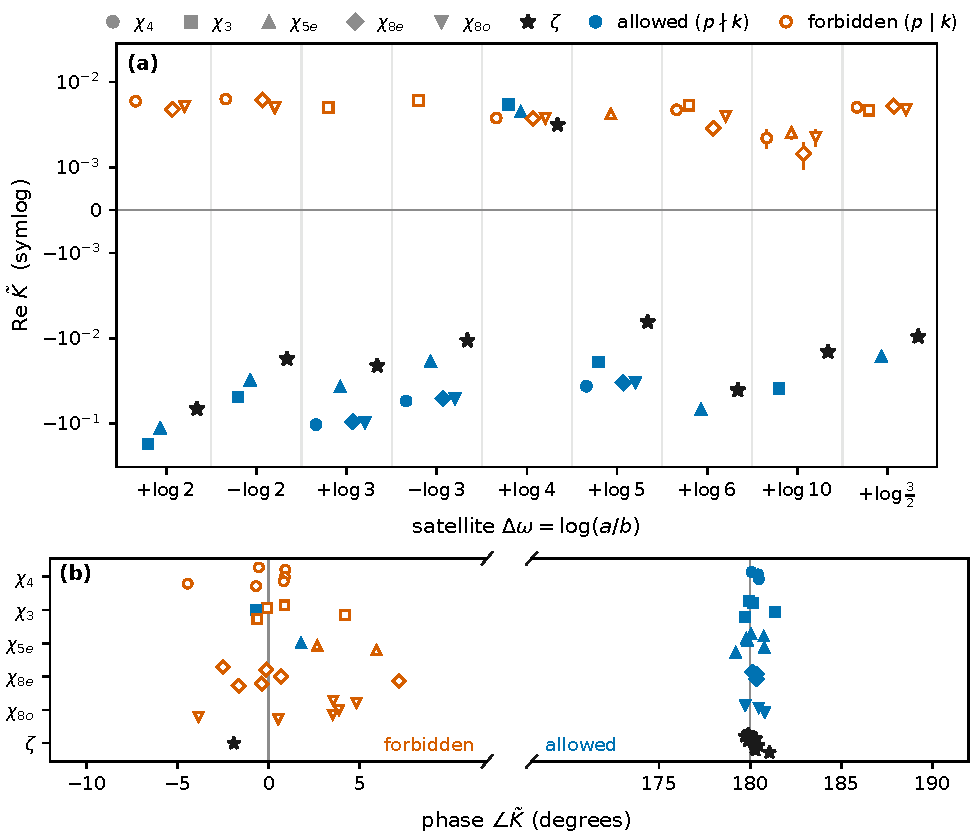
\includegraphics[width=0.95\textwidth]{fig_n7_characters_en.pdf}
\caption{\label{fig:chars}\textbf{The character selects the satellites of Dirichlet $L$-function zeros.}
  (a)~$\mathrm{Re}\,\tilde K$ (symlog scale, jackknife errors) at nine satellites for five
  islands of zeros ($\chi_4,\chi_3,\chi_{5e},\chi_{8e},\chi_{8o}$; $L_\chi\ge8.5$) and for
  $\zeta$ (stars; low window on the same $\Delta L$ block grid); filled symbols are allowed
  satellites ($n=a/b$ has no prime factor $p\mid k$), open symbols forbidden ones.
  Allowed satellites with $\mu(a)\neq0$ carry the sign of $\zeta$ in both parities
  ($z=-55$ to $-82$ for the six primary pairs; $\chi_{8o}/\chi_{8e}=1.009\pm0.024$ at
  $+\log3$), whereas forbidden satellites leave only a small residual of opposite sign,
  $+0.0014$ to $+0.0063$, at the level of the $\mu(4)=0$ position $+\log4$ (positive also
  for $\zeta$, $\chi_3$ and $\chi_{5e}$).
  (b)~Phases: $\angle\tilde K=180^\circ\pm1.3^\circ$ for every allowed $\mu\neq0$ satellite,
  odd or even, and $0^\circ\pm7.2^\circ$ for every forbidden one.}
\end{figure}

\section{The Bogomolny--Keating mirror law}\label{sec:BK}

The first-order amplitude rule of Derivation~\ref{der:sp} ---
brightness $\propto |\mu(n)|/\varphi(n)$ on the positive side and
$\propto 1/m$ at $n = 1/m$ --- gets the ordering of the satellites right
but not their magnitudes: odd primes fade faster than predicted. The
amplitudes are instead given by the Bogomolny--Keating pair correlation
\cite{BK95,BK96,Bog07}, re-derived from the ratios conjecture by Conrey
and Snaith \cite{CS07}, whose off-diagonal part is, in the form of
\cite[eqs.~(7.5)--(7.6)]{Bog07},
\begin{equation}\label{eq:BK}
R_2^{\mathrm{off}}(\varepsilon) \propto e^{iL\varepsilon}\,
|\zeta(1+i\varepsilon)|^2\,\Phi(\varepsilon) + \mathrm{c.c.},\qquad
\Phi(\varepsilon) = \prod_p\Big[1 - \frac{(1-p^{i\varepsilon})^2}{(p-1)^2}\Big].
\end{equation}
The carrier $e^{iL\varepsilon}$ places the structure on the comb; the
envelope $f = |\zeta(1+i\varepsilon)|^2\Phi$ is an Euler product,
$f = \prod_p g_p(\varepsilon\log p)$ with
$g_p(\theta) = |1 - e^{-i\theta}/p|^{-2}\,[1 - (1 - e^{i\theta})^2/(p-1)^2]$,
and its Bohr coefficient at frequency $\log r$ (the coefficient of
$e^{i\varepsilon\log r}$ in its almost-periodic expansion) is the amplitude
of the satellite $\Delta\omega = \log r$.

\begin{derivation}[Closed form]\label{der:closed}
The first factor of $g_p$ has Fourier coefficients
$A_k = p^{-|k|}/(1 - p^{-2})$; the second is a trigonometric polynomial with
coefficients $B_0 = 1 - (p-1)^{-2}$, $B_1 = 2(p-1)^{-2}$,
$B_2 = -(p-1)^{-2}$. Hence $\hat g_p(k) = \sum_j B_j A_{k-j}$, and
\[
\frac{\hat g_p(k)}{\hat g_p(0)} =
\begin{cases} p^{k}, & k \le 0,\\ p/(p-1)^2, & k = 1,\\ 0, & k\ge 2,\end{cases}
\]
the last because $\hat g_p(k) \propto p^{-k}(B_0 + pB_1 + p^2 B_2) = 0$.
The satellite at $\log r$, $r = \prod_p p^{k_p}$ in lowest terms, has
relative amplitude $c(r) = \prod_p f_p(k_p)$ with $f_p$ the right-hand
side.
\end{derivation}

Three consequences. \emph{Mirror law}: on the negative side,
$c(1/n) = 1/n$ for every integer $n$ and $c(2/m) = 2/m$ for odd $m$, so the
envelope at $\Delta\omega = -\log x$ is exactly $1/x$ on the half-integers;
between them, satellites $x = b/3$ and $x = b/6$ lie on a quarter envelope
$0.25/x$, and all other families are below $0.03$. \emph{Prime-power
asymmetry}: $+\log p^k$ with $k\ge2$ is exactly dark (as the selection rule
of Section~\ref{sec:classes} says), but $-\log p^k$ is bright.
\emph{Positive side}: $c(p) = p/(p-1)^2$, so $c(2) = 2$, $c(3) = 3/4$,
$c(5) = 5/16$, $c(7) = 7/36$; the factor $f_2(1) = 2$ explains why
$+\log 2m$ is twice as bright as $+\log m$ for odd $m$.

\subsection*{A lesson in line shape (post hoc)}
Compared with the 23 satellite amplitudes of the first catalogue (eight
blocks, point readings, normalised to $+\log2$), the closed form fits the
mirror side ($-\log 2$: $0.96$, $-\log 3$: $1.05$ of the prediction) but
misses several mixed ratios by $3$--$10\sigma$, one of them with the wrong
sign ($+\log(5/3)$). With 32 blocks and profile fits these misses largely
disappear ($+\log(5/3)$: $-0.44 \to +0.42$; $+\log(5/2)$: $0.17\to0.57$;
$-\log(4/3)$: $0.31\to0.79$): they were produced by the eight-block line
shape, whose width exceeds the satellite spacing.

\subsection*{The blind test}
The mirror law was tested in the band $-2.12 \le \Delta\omega \le -1.58$
($4.86 \le x \le 8.33$), whose part below $-1.775$ had never been computed and whose
remainder had been computed in an earlier map but never displayed or
searched (no figure or search had gone below $-1.35$). The test was
pre-registered after an independent derivation audit; its design was
changed several times before the data were seen, each time because an
audit or a synthetic power study showed a weakness.

The final design fits the band with the seven main satellites free, the quarter-envelope satellites
fixed from a calibration window on the seen side, and a linear baseline.
It compares two hypotheses by self-consistency: \emph{BK} (amplitudes
$s/x$, with the scale $s$ fixed by $-\log 2$ and $-\log 3$) and a rival in
which the amplitude also carries the smooth line-density factor
$e^{\omega'/2}/\omega'$ (predicting $0.71$ of BK in the band). In $2\times200$
synthetic replicas the correct hypothesis won in $93\%$ and $86\%$ of
cases and the wrong one in at most $0.5\%$.

\begin{observation}[Mirror law; blind]\label{obs:mirror}
In the low window, the ratios $R_x = A_x/(s/x)$ of the integer family are
$1.016\pm0.018$, $1.014\pm0.033$, $1.046\pm0.031$, $1.048\pm0.060$ for
$x = 5, 6, 7, 8$; their weighted mean is $1.023\pm0.023$, and the rival is
excluded at more than $12\sigma$. The prime power $x = 8$ lies on the
envelope ($0.993\pm0.039$ of the fitted $x^{-\beta}$ law), although
$+\log 8$ is dark. The half-integer family ($x = 5.5, 6.5, 7.5$) lights up
at $0.789\pm0.037$ of the integer family --- inside the pre-registered
band $|\rho - 1|\le 0.25$, but significantly below one.
\end{observation}

\begin{figure}[t]
\centering
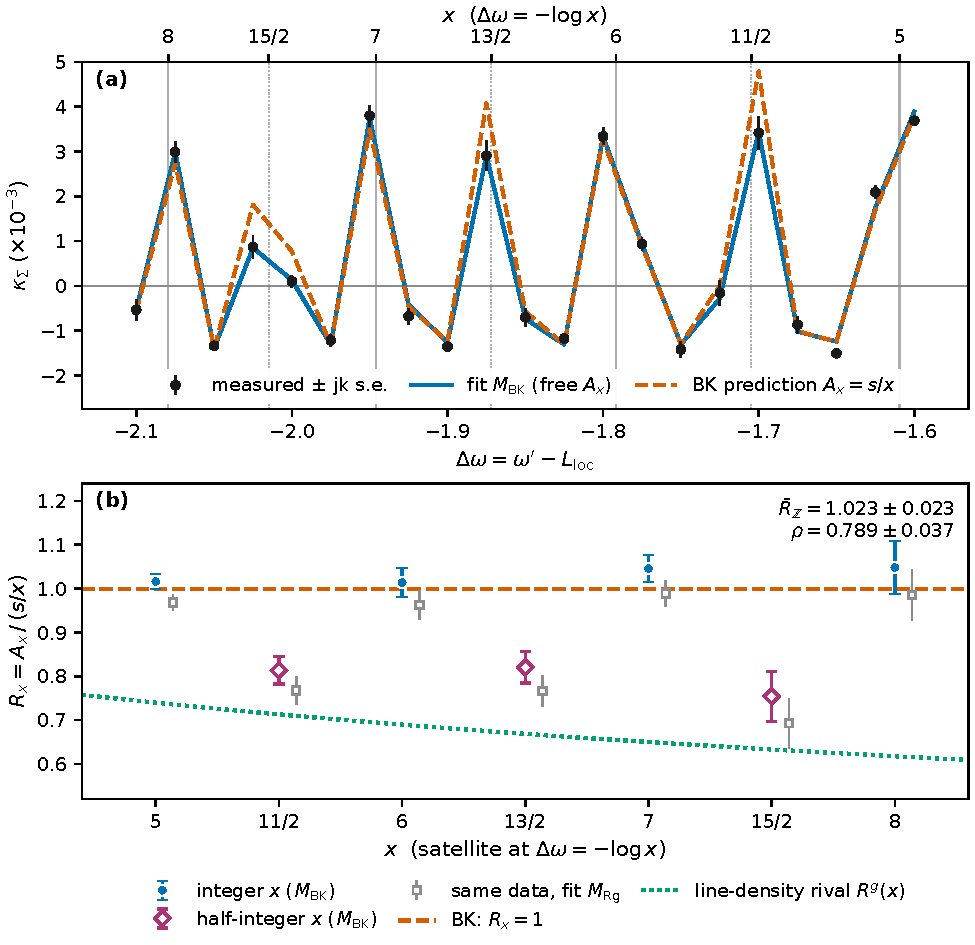
\includegraphics[width=0.95\textwidth]{fig_n7_mirror_en.pdf}
\caption{\label{fig:mirror}\textbf{Mirror law in the blind band.}
  (a)~Kernel $\kappa_\Sigma$ (32 blocks, window $L=10.48$, jackknife errors) in the
  pre-registered, previously unviewed band $-2.12\le\Delta\omega\le-1.58$, with the
  free-amplitude fit $M_{\rm BK}$ and the parameter-free Bogomolny--Keating prediction
  $A_x=s/x$ ($s$ from the calibration band $-1.30\le\Delta\omega\le-0.55$; same linear
  baseline and fixed quarter-family terms); solid and dotted grid lines mark integer and
  half-integer $x$ at $\Delta\omega=-\log x$.
  (b)~Amplitude ratios $R_x=A_x/(s/x)$: the integer family gives
  $\bar R_{\mathbb Z}=1.023\pm0.023$ ($\sigma_{\rm eff}$), whereas the line-density rival
  predicts $\bar R^g=0.706$ and its own fit (grey) returns $0.972$, more than
  $12\sigma_{\rm eff}$ away.
  The half-integer family follows the same $1/x$ envelope at a reduced level,
  $\rho=0.789\pm0.037$, and the prime power $x=8$ is not suppressed
  ($R_8=1.048\pm0.060$, $\psi=0.993\pm0.039$).}
\end{figure}

\section{Positive exponents and height}\label{sec:height}

Relative to the mirror scale of the same window, the positive-exponent
coefficients are transferred with a factor below one. In the low window
$\eta_p := A(+\log p)/(s\,c(p))$ is $0.79$, $0.71$, $0.60$, $0.54$ for
$p = 2, 3, 5, 7$, and the same factors account, approximately
multiplicatively, for the half-integer family ($\eta_2$), the
quarter-envelope families ($\eta_3$, $\eta_2\eta_3$) and the mixed
ratios. A post-hoc look suggested $\eta_p \approx p^{-1/3}$. Whether this
is a constant or a finite-height effect was pre-registered as a test over
three windows, with the model $1 - \eta_p(L) = B_p (L/L_0)^{-\gamma}$:
$\gamma = 1$ for a correction of relative order $1/L$, $\gamma = 0$ for a
constant.

\begin{table}[h]
\centering
\begin{tabular}{lcccccc}
\toprule
window & $L$ & $\eta_2$ & $\eta_3$ & $\eta_5$ & $\eta_7$ \\
\midrule
alt (blind) & $9.34$ & $0.784(14)$ & $0.663(13)$ & $0.583(19)$ & $0.521(28)$\\
low & $10.48$ & $0.789(11)$ & $0.713(15)$ & $0.604(21)$ & $0.538(20)$\\
last & $12.03$ & $0.837(9)$ & $0.770(7)$ & $0.712(14)$ & $0.616(26)$\\
\bottomrule
\end{tabular}
\caption{\label{tab:kappa}Positive-exponent transfer factors in three
windows (jackknife errors in the last digits). The alt window is fully
blind; coarse satellite ratios of the last window had been seen before
the test (see text).}
\end{table}

\begin{observation}[Height dependence; pre-registered]\label{obs:height}
The common exponent is $\gamma = 1.36\pm0.21$; a constant is excluded at
$6.4\sigma$. The ratio of the last to the alt window, which does not use
the window in which the pattern was first seen, excludes a constant at
$7.9\sigma$ (and is $1.9\sigma$ steeper than $\gamma = 1$). The half-integer
families relax towards one in the same way ($R(5/2)$: $0.79\to0.83\to0.92$;
$R(7/2)$: $0.75\to0.81\to0.88$), as does the quarter envelope
($0.65\to0.69\to0.75$), while the integer mirror side stays at one in all
windows.
\end{observation}

Two caveats belong with this result. The decisive leverage comes from the
last window, whose coarse ratios had been seen (without distinguishing
the hypotheses) in an earlier test; the fully blind alt window alone gives
$1.074\pm0.055$ against $1.122$ ($\gamma=1$) and $1$ ($\gamma=0$), as the
power study had anticipated. And three windows cannot fix the functional
form: the change is small between $L = 9.3$ and $10.5$ and large between
$10.5$ and $12.0$. The $p^{-1/3}$ pattern was a coincidence of height.

The negative residues at the positions with $\mu(a)=0$
(Section~\ref{sec:classes}) do not relax: in units of the mirror scale
they are $-0.023$, $-0.023$, $-0.032$ at $+\log4$, $-0.021$, $-0.018$,
$-0.017$ at $+\log 8$ and $-0.020$, $-0.016$, $-0.020$ at $+\log 9$ in the
alt, low and last windows.

What does the height dependence mean? The Conrey--Snaith pair correlation
contains all lower-order arithmetic terms, with an error
$O(T^{1/2+\varepsilon})$ \cite{CS07}, and its carrier term has
$L$-independent Bohr coefficients. The relaxation is therefore not a
correction to \eqref{eq:BK}; it is a property of the way our mixed
zero--prime observable transfers the coefficients of $R_2$ --- exactly on
the negative side, and only asymptotically on the positive side.

\begin{figure}[t]
\centering
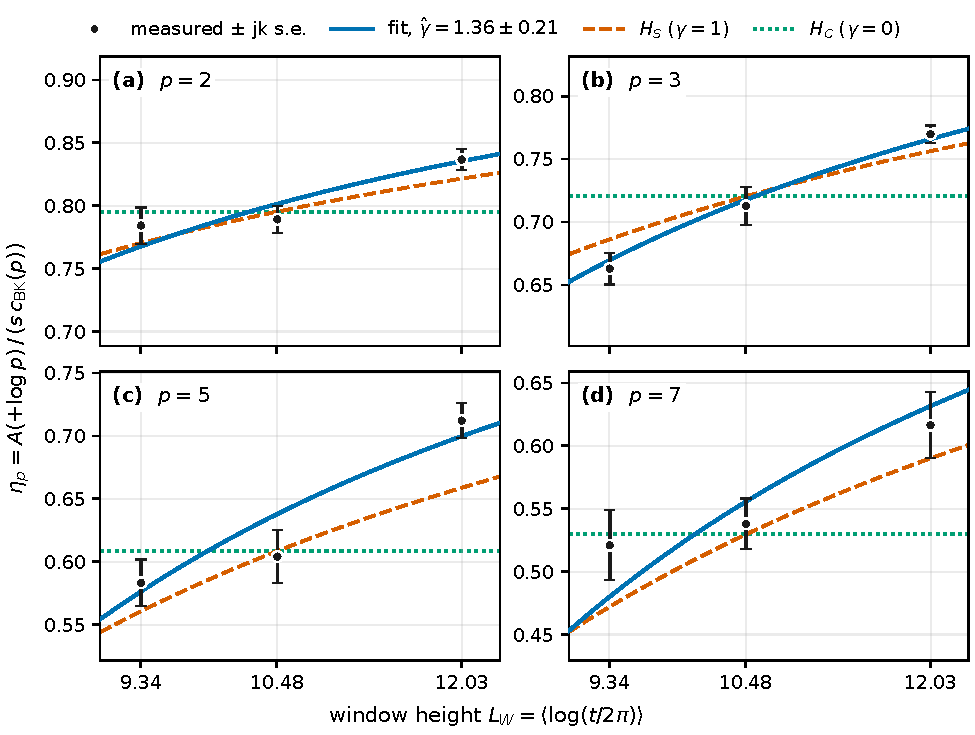
\includegraphics[width=0.95\textwidth]{fig_n7_height_en.pdf}
\caption{\label{fig:height}\textbf{Height dependence of the positive-exponent factors.}
  $\eta_p=A(+\log p)/(s\,c_{\rm BK}(p))$ for $p=2,3,5,7$ in three windows,
  $L_W=9.34$ (blind), $10.48$ (reference) and $12.03$, with jackknife errors.
  Solid: joint fit $1-\eta_p=B_p(L/L_d)^{-\gamma}$ with $L_d=10.48$, giving
  $\hat\gamma=1.36\pm0.21$ ($\sigma_{\rm eff}$); dashed: finite-height hypothesis $H_S$
  ($\gamma=1$); dotted: constant structure $H_C$ ($\gamma=0$), both anchored at the
  pre-registered values $\eta_p=0.795,\,0.720,\,0.608,\,0.530$ (the first,
  32-block measurement; the low-window values of Table~\ref{tab:kappa} use
  equal-$\Delta L$ blocks).
  $\hat\gamma$ lies $1.7\sigma$ from $H_S$ and $6.4\sigma$ from $H_C$: the factors relax
  towards the Bogomolny--Keating value $\eta_p=1$ as the height grows.}
\end{figure}

\section{Open problems}\label{sec:open}

\begin{enumerate}
\item \emph{The transfer function.} Derive $\eta_p(L)$ from the
definition \eqref{eq:K} and the identity \eqref{eq:ds}: why is the
transfer exact for negative exponents and asymptotic for positive ones?
\item \emph{The $\mu = 0$ residues.} Positions where the closed form is
exactly zero carry negative residues of about $2\%$ of the mirror scale,
independent of height, and the conductor-forbidden satellites of
$L$-functions carry residues at the same level. Are they a term beyond
\eqref{eq:BK}?
\item \emph{Magnitudes.} The class shares of $+\log 7$ and $+\log 5$
exceed \eqref{eq:shares} by factors $1.25$--$2.4$, and the $L$-function
amplitudes follow $(k/\varphi(k))\prod J_0$ rather than
$\sqrt{k}/\varphi(k)$. Neither is derived.
\item \emph{Half-integers.} The half-integer family sits at $\approx0.8$
of the mirror law and relaxes with height like $\eta_2$; is it
$\eta_2$?
\end{enumerate}

A recent preprint \cite{Kan26} reports no detectable arithmetic
frequencies in the deviations of $\Delta_3$ from random-matrix theory.
We note that on the unfolded axis used there the arithmetic frequencies
sit at $2\pi\log p/\log(T/2\pi)$ rather than at $\log p$, which may account
for the null result; the satellites reported here are, in any case, a
different observable.

\section*{Reproducibility}

All code, data products, pre-registration files (with sha256 stamps and
the dates at which they were published) and the research log, including
the failed predictions, are available in the repository
\url{https://github.com/azizran/riemann-zero-statistics} (directory
\texttt{qm\_riemann/}; Section~\ref{sec:pos}: tasks 188, 190;
Section~\ref{sec:classes}: 192--194; Section~\ref{sec:L}: 195;
Section~\ref{sec:BK}: 196--197; Section~\ref{sec:height}: 198), archived at Zenodo,
\href{https://doi.org/10.5281/zenodo.22942475}{doi:10.5281/zenodo.22942475}.

\section*{Acknowledgements}

Computational assistance, derivation audits, literature search and
drafting: Claude (Anthropic); pre-registrations were audited by an
independent model instance before predictions were frozen. Errors are
the author's.

\begin{thebibliography}{99}

\bibitem{companion1} U.~Sezen, \emph{The joint law of zero gaps and local
maxima of Hardy's $Z$-function}, preprint (2026); archived at Zenodo,
\href{https://doi.org/10.5281/zenodo.22942475}{doi:10.5281/zenodo.22942475}.

\bibitem{companion2} U.~Sezen, \emph{The prime-wave anatomy of the
gap--amplitude law for Riemann zeros}, preprint (2026); archived at Zenodo,
\href{https://doi.org/10.5281/zenodo.22942475}{doi:10.5281/zenodo.22942475}.

\bibitem{companion3} U.~Sezen, \emph{A response theory for the Riemann
zero gas}, preprint (2026); archived at Zenodo,
\href{https://doi.org/10.5281/zenodo.22942475}{doi:10.5281/zenodo.22942475}.

\bibitem{companion4} U.~Sezen, \emph{The Riemann zero lattice as a warm
crystal}, preprint (2026); archived at Zenodo,
\href{https://doi.org/10.5281/zenodo.22942475}{doi:10.5281/zenodo.22942475}.

\bibitem{BK95} E.~B.~Bogomolny, J.~P.~Keating, \emph{Random matrix theory and the
Riemann zeros I: three- and four-point correlations}, Nonlinearity \textbf{8}
(1995), 1115--1131.

\bibitem{BK96} E.~B.~Bogomolny, J.~P.~Keating, \emph{Random matrix theory and the
Riemann zeros II: $n$-point correlations}, Nonlinearity \textbf{9} (1996), 911--935.

\bibitem{Bog07} E.~Bogomolny, \emph{Riemann zeta function and quantum chaos},
Prog.\ Theor.\ Phys.\ Suppl.\ \textbf{166} (2007), 19--36, arXiv:0708.4223.

\bibitem{CS07} J.~B.~Conrey, N.~C.~Snaith, \emph{Applications of the $L$-functions
ratios conjectures}, Proc.\ London Math.\ Soc.\ (3) \textbf{94} (2007), 594--646,
arXiv:math/0509480.

\bibitem{Mont73} H.~L.~Montgomery, \emph{The pair correlation of zeros of the zeta
function}, in: Analytic Number Theory, Proc.\ Sympos.\ Pure Math.\ \textbf{24},
Amer.\ Math.\ Soc., Providence, RI, 1973, 181--193.

\bibitem{Rod13} B.~Rodgers, \emph{Macroscopic pair correlation of the Riemann
zeroes for smooth test functions}, Q.\ J.\ Math.\ \textbf{64} (2013), 1197--1219,
arXiv:1203.3275.

\bibitem{Landau12} E.~Landau, \emph{\"Uber die Nullstellen der Zetafunktion},
Math.\ Ann.\ \textbf{71} (1912), 548--564.

\bibitem{Gonek93} S.~M.~Gonek, \emph{An explicit formula of Landau and its
applications to the theory of the zeta-function}, in: M.~Knopp et al.\ (eds.), A
Tribute to Emil Grosswald: Number Theory and Related Analysis, Contemp.\ Math.\
\textbf{143}, Amer.\ Math.\ Soc., Providence, RI, 1993, 395--413.

\bibitem{Fujii89} A.~Fujii, \emph{On a theorem of Landau}, Proc.\ Japan Acad.\ Ser.\
A Math.\ Sci.\ \textbf{65} (1989), no.~2, 51--54.

\bibitem{DHPC26} B.~Durkan, C.~Hughes, A.~Pearce-Crump, \emph{Generalisations of the
Landau--Gonek theorem and applications to mean values of zeta}, arXiv:2601.18025
[math.NT] (2026), preprint.

\bibitem{ZMT18} G.~Zhang, F.~Martelli, S.~Torquato, \emph{The structure factor of
primes}, J.\ Phys.\ A: Math.\ Theor.\ \textbf{51} (2018), 115001, arXiv:1801.01541.

\bibitem{TZdCI18} S.~Torquato, G.~Zhang, M.~de Courcy-Ireland, \emph{Uncovering
multiscale order in the prime numbers via scattering}, J.\ Stat.\ Mech.\ Theory Exp.\
\textbf{2018} (2018), 093401, arXiv:1802.10498.

\bibitem{Odl87} A.~M.~Odlyzko, \emph{On the distribution of spacings between zeros
of the zeta function}, Math.\ Comp.\ \textbf{48} (1987), 273--308.

\bibitem{OdlyzkoTables} A.~M.~Odlyzko, \emph{Tables of zeros of the Riemann zeta
function}, \url{https://www-users.cse.umn.edu/~odlyzko/zeta_tables/}.

\bibitem{Apo76} T.~M.~Apostol, \emph{Introduction to Analytic Number Theory},
Undergraduate Texts in Mathematics, Springer-Verlag, New York--Heidelberg--Berlin,
1976.

\bibitem{Kan26} S.~Kanivets, \emph{No Evidence for Detectable Arithmetic
Frequencies in Long-Range Deviations of Riemann Zero Statistics from Random Matrix
Theory}, Zenodo (2026), \url{https://doi.org/10.5281/zenodo.20766728}.

\end{thebibliography}

\end{document}
